% Suggested outline when preparing the Qualifying Examination research presentation:
% 1.What is the research problem? Why is it hard? Who does it impact?
% 2.How is it solved today? What are the limits of current practice?
% 3.What is the new technical idea?
% Why we can succeed now?
% 4.Are there others dedicated to finding a solution to the problem?
% 5.What is the impact if successful?

\documentclass{beamer}
\usepackage{graphicx}
\usepackage[utf8]{inputenc}
\usepackage{amsmath, amssymb}

%Information to be included in the title page:
\title{Software Reusability in Autonomous Vehicle Steering}
\author{Emiko Soroka\\PI: Sanjay Lall}
\institute{Stanford University}
\date{\today}
\pagenumbering{arabic}
\setbeamertemplate{footline}[frame number] 

\begin{document}
	
	\frame{\titlepage}
	
	% 1.What is the research problem? Why is it hard? Who does it impact?
\begin{frame}
\frametitle{Software Reusability: A Growing Problem}
Advanced driver assistance systems (ADAS) and autonomous vehicles are a rapidly growing segment of the automotive industry
\begin{columns}
	\begin{column}{0.5\linewidth}
\begin{figure}
	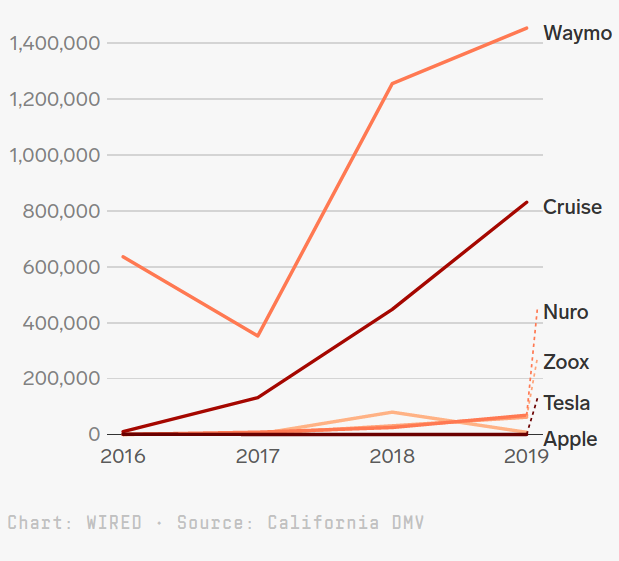
\includegraphics[width=1.0\linewidth]{figures/miles_driven_waymo.png}
	\caption{Autonomous miles driven by top California companies}
\end{figure}
	\end{column}
	\begin{column}{0.45\linewidth}
\begin{figure}
	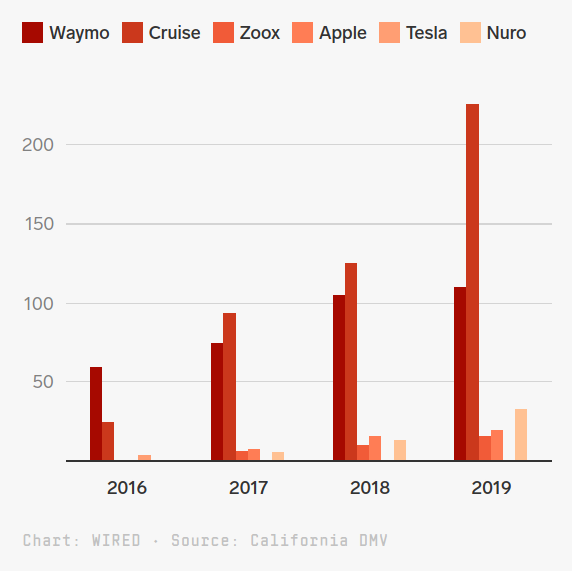
\includegraphics[width=1.0\linewidth]{figures/miles_by_autonomous_cars.png}
	\caption{Number of self-driving vehicles on the road}
\end{figure}
\end{column}
\end{columns}

\tiny(Chart source:\ \texttt{https://www.wired.com/story/california-self-driving-cars-log-most-miles/})
\normalsize
\end{frame}

\begin{frame}
\frametitle{Software Reusability: A Growing Problem}
The rise of autonomous driving comes with new challenges in software reusability.
\begin{itemize}
	\item Port an existing autonomous driving stack to different vehicles
	\item Verify safety-critical software operates correctly on different platforms.
	\item Comply with regulations and standards.
\end{itemize}
\begin{figure}
	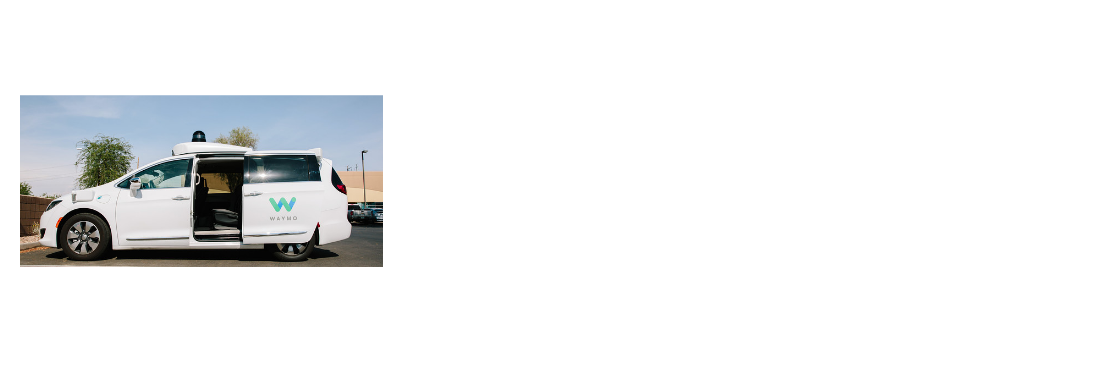
\includegraphics[width=0.9\linewidth]{figures/one.png}
\end{figure}
\end{frame}

\begin{frame}
\frametitle{Software Reusability: A Growing Problem}
The rise of autonomous driving comes with new challenges in software reusability.
\begin{itemize}
	\item Port an existing autonomous driving stack to different vehicles
	\item Verify safety-critical software operates correctly on different platforms.
	\item Comply with regulations and standards.
\end{itemize}
\begin{figure}
	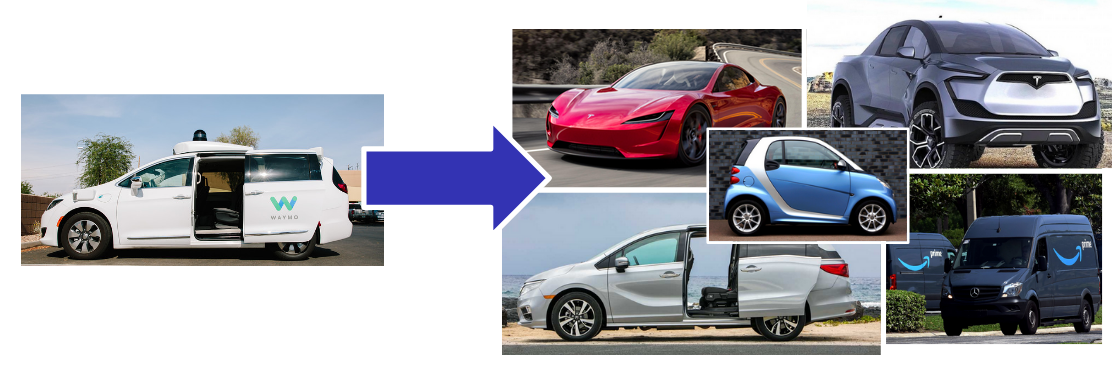
\includegraphics[width=0.9\linewidth]{figures/one_to_many.png}
\end{figure}
\end{frame}


\begin{frame}
\frametitle{Software Portability in the Autonomy Stack}

\begin{columns}
	\begin{column}{0.5\linewidth}
High-level software (route planning, computer vision) is easily ported to different vehicles.
		% such as route planning, computer vision, and other high-level processes.
		
		However, low-level control depends on vehicle-specific hardware for multiple reasons.
		\begin{itemize}
			\item Fuel efficiency
			%hybrid vehicle vs electric vehicle, regenerative braking.
			\item Physical parameters
			\item Vehicle dynamics
			%weight, center of gravity (CG), tire size and tire-road interactions.
			\item Engine performance
			% (number of cylinders, front-wheel drive vs all-wheel drive, etc).
		\end{itemize}
		\end{column}
	\begin{column}{0.45\linewidth}
		\begin{figure}
			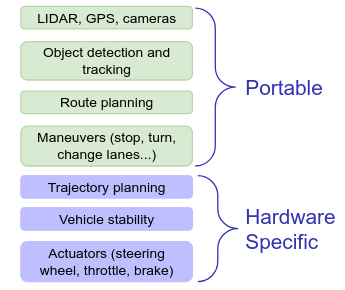
\includegraphics[width=1.0\linewidth]{figures/autonomy_stack_small.png}
			% Comment: This is a standard autonomy stack
		\end{figure}
	\end{column}
\end{columns}
\vspace{1.0em}

In this presentation, we focus on steering and acceleration control. Our goal is to \textbf{disentangle hardware-dependent control algorithms from higher-level software.}
\end{frame}

\begin{frame}
\frametitle{Steering an Autonomous Vehicle}
Major concerns when steering an autonomous vehicle:
\begin{itemize}
\item Safety: vehicle must not lose control or stray from a safe path.
\item Comfort: Steer and accelerate smoothly, reducing jerk (change in acceleration).
\item Fuel efficiency: avoid unnecessary control inputs.
\end{itemize}

However, not all applications weight these equally.
\begin{itemize}
\item Autonomous delivery truck: maximize fuel efficiency.
\item Autonomous taxi: provide a comfortable and enjoyable ride.
\end{itemize}
%Configurable behavior is already on the market: many ADAS systems allow switching between ``sport" and ``eco-friendly" driving modes.

\begin{figure}
	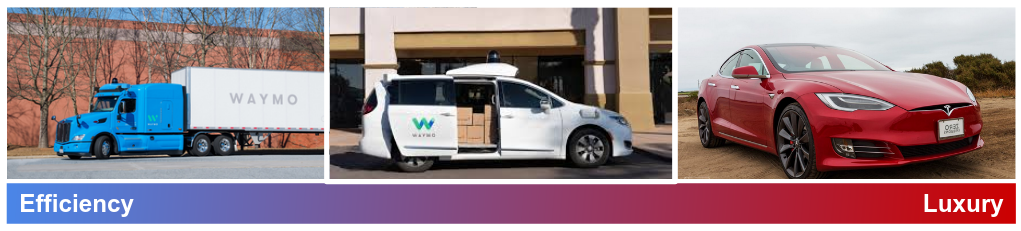
\includegraphics[width=1.0\linewidth]{figures/configurability.png}
\end{figure}
\end{frame}

% UNNECESSARY TO HAVE THIS SLIDE
% Just talk in words about modal changes (Lall's word) such as trucks driving different from cars.
%	\begin{frame}
%\frametitle{Software reusability perspective}
%Changing behavior is also a high-level goal.
% COMMENT: Is this a digression?
%\begin{columns}
%	\begin{column}{0.65\linewidth}
%\begin{itemize}
%	\item What speed does the vehicle drive at?
%	\item What lane does it drive in?
%\end{itemize}
%	\end{column}
%\begin{column}{0.35\linewidth}
%		\begin{figure}
%	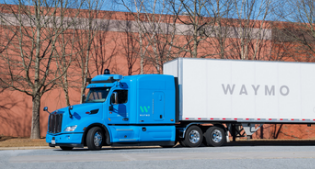
\includegraphics[width=1.0\linewidth]{figures/waymo_truck.png}
%\end{figure}
%\end{column}
%\end{columns}
%\vspace{1.0em}
%However, to plan these behaviors the autonomy software must know what its hardware is capable of.
%\begin{itemize}
%	\item If our trajectory planner is platform-independent, it can't take advantage of the full %capabilities of the hardware.
%	
%	\item If our planner is hardware-dependent, it will be difficult to port the software to new %vehicles.
%\end{itemize}

%\end{frame}
% 2.How is it solved today? What are the limits of current practice?


\begin{frame}
\frametitle{Literature review}

TODO: (How to handle citations???)
\end{frame}

\begin{frame}
	\frametitle{Trajectory Tracking with Waypoints}
In trajectory tracking (as opposed to trajectory planning or optimization), the goal is to follow a given path as closely as possible. Many approaches are possible, including	PID and tracking MPC.

Challenges with trajectory tracking:
	\begin{itemize}
		\item Tuning PID gains
		\item Proving a PID controller is stable
		\item Developing controllers for complex vehicle models that represent the interactions between tires, axles, vehicle body, suspension, etc.
	\end{itemize}
\textbf{Problem: A higher-level module must have enough information about vehicle hardware to generate the waypoints.}
\end{frame}
	
	% 3.What is the new technical idea?
\begin{frame}
\frametitle{Trajectory Optimization: Beyond Waypoints?}
Some controllers optimize the vehicle's trajectory: for example, by determining the best path in a safe driving corridor.
\vspace{1em}
\begin{columns}
	\begin{column}{0.6\linewidth}
High-level software could provide this safe corridor and driving goals. The exact path is determined by the steering controller.
	\end{column}
	\begin{column}{0.3\linewidth}
	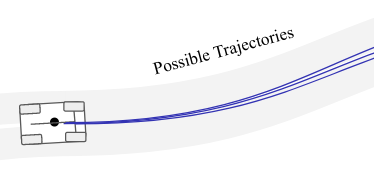
\includegraphics[width=1.0\linewidth]{figures/many_trajectories.png}
\end{column}
\end{columns}
\vspace{1em}

Some challenges with this approach:
\begin{itemize}
	\item Nonlinear dynamics add difficulty to the optimization problem.
	\item The safe corridor the vehicle can drive in is difficult to represent.
	\item The dynamics model must be computationally tractable.
	\item The optimization must run in real time.
\end{itemize}
\end{frame}
\begin{frame}
\frametitle{Example Applications}
\begin{itemize}
	\item Dynamic maneuvers such as emergency braking / steering
	\begin{itemize}
		\item Requires accurate knowledge of hardware capabilities
	\end{itemize}
	\item Stopping at a stop sign (an interesting problem)
	\begin{itemize}
		\item How do we represent the constraint that the vehicle must stop at a certain position?
		\item The velocity can change, so we don't know which time step the stop will occur at.
	\end{itemize}
\end{itemize}
\begin{figure}
	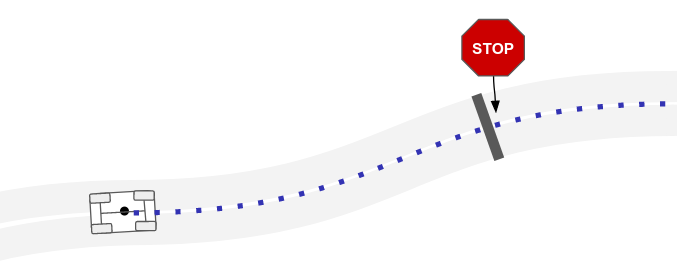
\includegraphics[width=0.6\linewidth]{figures/stop_sign.png}
\end{figure}
% Another thing you can add to this slide is dynamic maneuvers, e.g. emergency braking, avoidance maneuvers, where the vehicle behavior is really complicated and one needs a really complicated model to execute those correctly.

% It's reasonable future self-driving cars will need this capability.
% TODO
\end{frame}

	

%\begin{frame}
%\frametitle{Improving Software Reusability}
%\begin{itemize}
%	\item Trajectory optimization allows higher-level autonomy software to operate with little knowledge of vehicle hardware.
	
%	\item High-level modules provide a goal (``drive at this speed", ``stop at the stop sign", ``slow down and take this exit off the highway") and constraints (a safe corridor to drive in, obstacles to avoid).
	
%	\item Lower-level optimization, with access to hardware parameters (possibly via estimation), computes control signals to meet this goal.
	
%	\item High-level software can be deployed quickly to a wide range of vehicles, while the low-level software is customized for specific platforms.
	
%	\item Providing a clean break between hardware independent and dependent software simplifies reusability and safety certification.
%\end{itemize}
%\end{frame}	

\begin{frame}
\frametitle{Proposed Division}
High-level software generates an inexact representation of the path without much knowledge of hardware capabilities.
% Knows basic information that informs mode changes: e.g. large delivery vehicles do not drive in the left lane, some vehicles limited to certain speed, etc.
\begin{itemize}
\item Provides a desired speed
\item Provides a safe driving corridor
\item Provides specific goals for low-level controller (stop at stop sign, hold constant speed on freeway)
\end{itemize}

Vehicle-specific controller optimizes this path.
\begin{itemize}
\item Accounts for hardware capabilities
\item Accounts for user preferences (comfort, fuel efficiency, etc.)
\end{itemize}
\vspace{-0.5em}
\begin{figure}
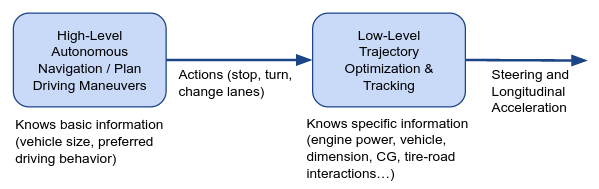
\includegraphics[width=0.8\linewidth]{figures/division.png}
\end{figure}
\end{frame}


\begin{frame}
\frametitle{MPC Trajectory Optimization}
Model-predictive control (MPC) is a good choice for the low-level controller.
\begin{itemize}
\item Weighting different objectives is an intuitive way to adjust driving behavior
\item Constraints can represent an allowable corridor to drive in, guaranteeing a trajectory won't violate safety requirements.
\item Vehicle kinematics models can be switched out without requiring major modifications to the controller.
\item Provides an abstraction to higher levels of the autonomy stack.
\end{itemize}

% TODO Talk explicitly about things that are constraints vs weights, stop at stop sign, etc.

\end{frame}

\begin{frame}
\frametitle{Trajectory Optimization Challenges}
Nonlinear optimization is difficult to implement.
\begin{itemize}
	\item Convergence to an optimal solution isn't guaranteed.
	\item In a complex problem, it can be difficult to determine why the solver failed or produced an unexpected result.
	\item Discretization of the vehicle dynamics and road corridor can introduce problems if not accurate enough.
\end{itemize}

Trade-off between model accuracy and computational tractability.
\begin{itemize}
	\item Even ``simple" models can be difficult to discretize.
	\item Adding complexity worsens this issue, but is necessary to handle a full range of driving conditions.%(example: knowledge of tire-road interactions is important in an emergency stop).
\end{itemize}
\end{frame}


\begin{frame}{Implementation of MPC controller}
\begin{figure}
	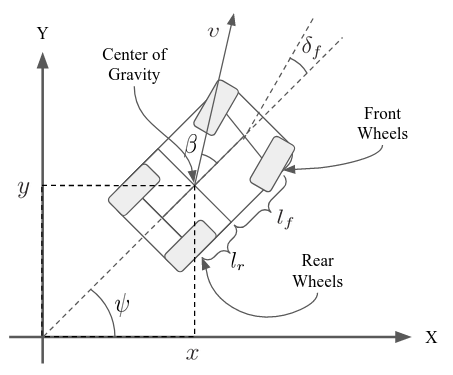
\includegraphics[width=0.38\linewidth]{figures/kinematic_diagram.png}
	\caption{Kinematic bicycle model, commonly used in MPC controllers.}
\end{figure}
\vspace{-0.5em}
\begin{equation}
\text{State } z = \begin{bmatrix}
x\\y\\v\\\psi
\end{bmatrix},\quad \begin{bmatrix}
\dot x\\\dot y\\\dot v\\\dot\psi
\end{bmatrix} = \begin{bmatrix}
v\cos(\psi + \beta)\\
v\sin(\psi + \beta)\\
a\\
\frac{v}{l_r}\sin(\beta)
\end{bmatrix}
\label{eq:kinematic}
\end{equation}
$\beta$ is the angle between the car velocity and its longitudinal axis \eqref{eq:beta}.

\begin{equation}
\beta = \tan^{-1}\Big( \frac{l_r}{l_f + l_r}\tan(\delta_f) \Big)
\label{eq:beta}
\end{equation}
\end{frame}

\begin{frame}
\frametitle{Implementation}
\begin{itemize}
\item Consider $N$ lookahead steps $k=1,\dots,N$ spaced $\Delta_t$ apart
\item The control signals are $a$, the longitudinal acceleration of the car, and $\delta_f$, the steering angle of its front wheels. $u = [a\ \delta_f]$
\item The nonlinearity is confined to the dynamics model \eqref{eq:kinematic}
\item The cost function is quadratic in state $z$ and control $u$
\item The state and control constraints are representable by linear inequalities
\end{itemize}
\vspace{-1.0em}
\begin{figure}
	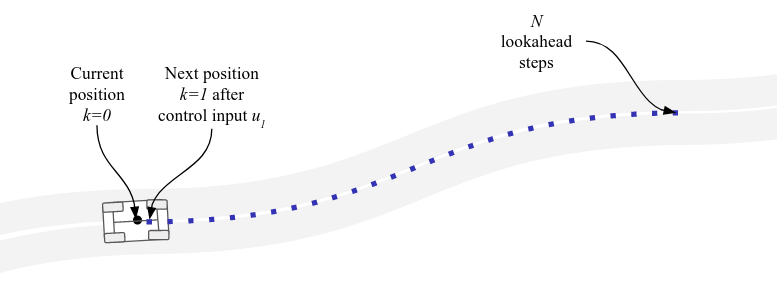
\includegraphics[width=0.9\linewidth]{figures/mpc_figure.png}
\end{figure}
\end{frame}



\begin{frame}
\frametitle{Implementation: Cost Function}
Define a multi-objective cost function. Changing the weights on each term will change the driving behavior.
\begin{equation}
J_{accuracy} = \sum_{k=1}^N\Big\| \begin{bmatrix}
x_k\\y_k\\\psi_k
\end{bmatrix} - \begin{bmatrix}
x_{center,k}\\y_{center,k}\\\psi_{center,k}
\end{bmatrix} \Big\|_2^2
\label{eq:costcenter}
\end{equation}
where $(x_{center,k}, y_{center,k}. \psi_{center,k}$ describe the $x-y$ position and angle of a desired point on the road (more on this later).
\begin{equation}
J_{speed} = \sum_{k=1}^N (v_k - v_{desired,k})^2
\label{eq:speed}
\end{equation}
Equation \eqref{eq:costcenter} controls the accuracy of the path-following behavior, while \eqref{eq:speed} controls how closely the vehicle stays at the desired speed.
\end{frame}

\begin{frame}
Equations \eqref{eq:costjerk} and \eqref{eq:coststeering} penalize undesirable sharp changes in acceleration and steering angle.
\frametitle{Implementation: Cost Function}
\begin{equation}
J_{jerk} = \sum_{k=2}^N (a_k - a_{k-1})^2
\label{eq:costjerk}
\end{equation}

\begin{equation}
J_{steering} = \sum_{k=2}^N (\delta_{f,k} - \delta_{f,k-1})^2
\label{eq:coststeering}
\end{equation}

Combine these terms to define the cost function:
\begin{equation}
J = a_1 J_{accuracy} + a_2 J_{speed} + a_3 J_{jerk} + a_4 J_{steering}
\label{eq:costfinal}
\end{equation}
\end{frame}

\begin{frame}
\frametitle{Implementation: MPC Problem}
Define the nonlinear MPC problem:
\begin{align}
\text{minimize}\quad& J(z_1,\dots,z_N, u_1,\dots,u_N)
\\
\text{subject to} \quad& z_{k} = f(z_{k-1}, u_{k-1}),\ k=1,\dots,N
\\
& u_{min} \leq u_k \leq u_{max},\ k=1,\dots,N
\\
& \begin{bmatrix}
v_{min}\\\psi_{min}
\end{bmatrix} \leq \begin{bmatrix}
v_k\\\psi_k
\end{bmatrix}\leq \begin{bmatrix}
v_{max}\\\psi_{max}
\end{bmatrix},\ k=1,\dots,N
\\
&
A_k\begin{bmatrix}
x_k\\y_k\\
\end{bmatrix} \geq 0,\ k=1,\dots,N
\end{align}
$A_k$ is the matrix of linear inequalities describing the road boundaries at the $k$th step.

The ``min" and ``max" bounds on $u,\ v$ and $\psi$ are constant.
\end{frame}

\begin{frame}
\frametitle{Implementation Challenges}
A major issue was representing the road accurately and efficiently.

Proposed solution: Use polygons to approximate the road at each step  $k=1,\dots,N$.
\vspace{-0.5em}
\begin{figure}
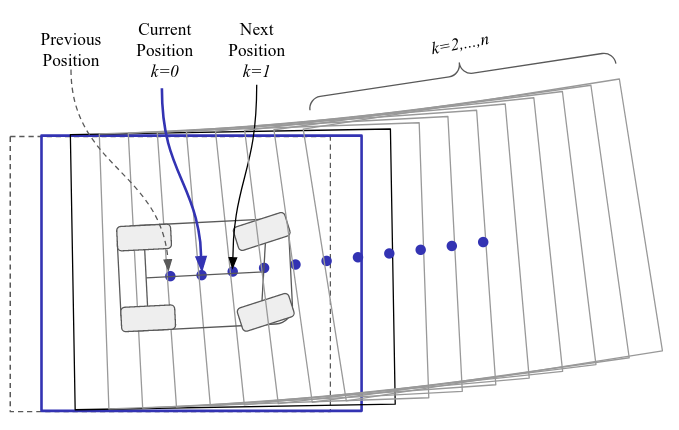
\includegraphics[width=0.7\linewidth]{figures/road_polygons.png}
\end{figure}
\vspace{-0.5em}
Then the position constraint on $x_k,y_k,\ k=1,\dots,N$ is simply a set of linear inequalities.
\end{frame}

\begin{frame}
\frametitle{Implementation Challenges}
This actually caused a lot of issues because it was difficult to generate the polygons without unnecessarily constraining the vehicle speed.
% A simplification I thought of to reduce coding issues (which loses the guarantee that the vehicle will stay in a bounded region, although in practice large accelerations are penalized) is to use the right and left boundaries, but leave the rear and front open.

Simplification: use the right and left boundaries, but leave the rear and front open.

\vspace{-0.5em}
\begin{figure}
	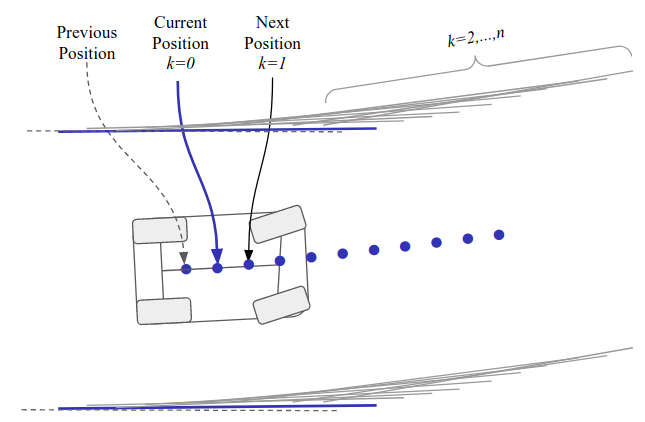
\includegraphics[width=0.7\linewidth]{figures/road_final_bounds.png}
\end{figure}
\vspace{-0.5em}

\end{frame}

\begin{frame}
\frametitle{Implementation Challenges}
Another major issue was formulating a cost function that causes the vehicle to move forward without  unnecessarily penalizing changes in velocity.

If we start with a (suboptimal) speed estimate, choosing points on the road center for steps $1,\dots,N$ without introducing ``noise" in the cost function is difficult.


\begin{figure}
	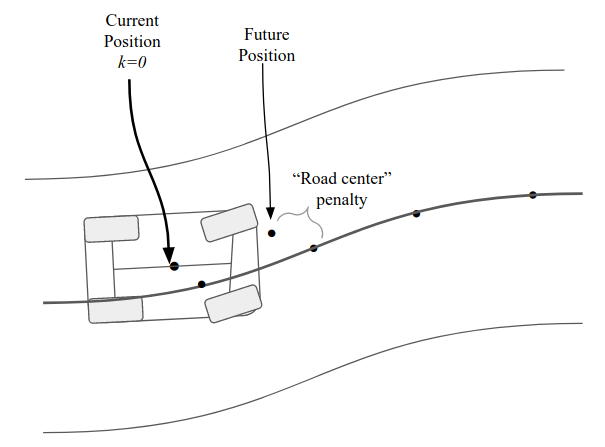
\includegraphics[width=0.55\linewidth]{figures/centering_issue.png}
\end{figure}
\vspace{-0.5em}

Solution: use previously computed trajectories to generate the center points.

\end{frame}


\begin{frame}
\frametitle{Performance on ISO Lane Change}
The ISO double lane change path is a test performed by human drivers on a real track, but is also used in some papers on autonomous driving.

The controller was implemented in Python using CasADi for symbolic math and Ipopt.
\begin{itemize}
	\item The linear boundaries successfully overlap to represent curved roads.
	\item The vehicle behavior can be changed using the weights on the cost terms.
	\item Because the road boundaries are a hard constraint,the vehicle cannot stray out of the road corridor. Deviations from the center of the road are only penalized, allowing it to make small adjustments to its path.
\end{itemize}
\end{frame}

\begin{frame}
\frametitle{Performance on ISO Lane Change}

In this slide, we see the results of several test runs. The ``accuracy" and ``speed" weights were successively increased: jerk and steering change weights remained the same at $100$ and $10$, respectively.

\vspace{-0.5em}
\begin{figure}
	\centering
	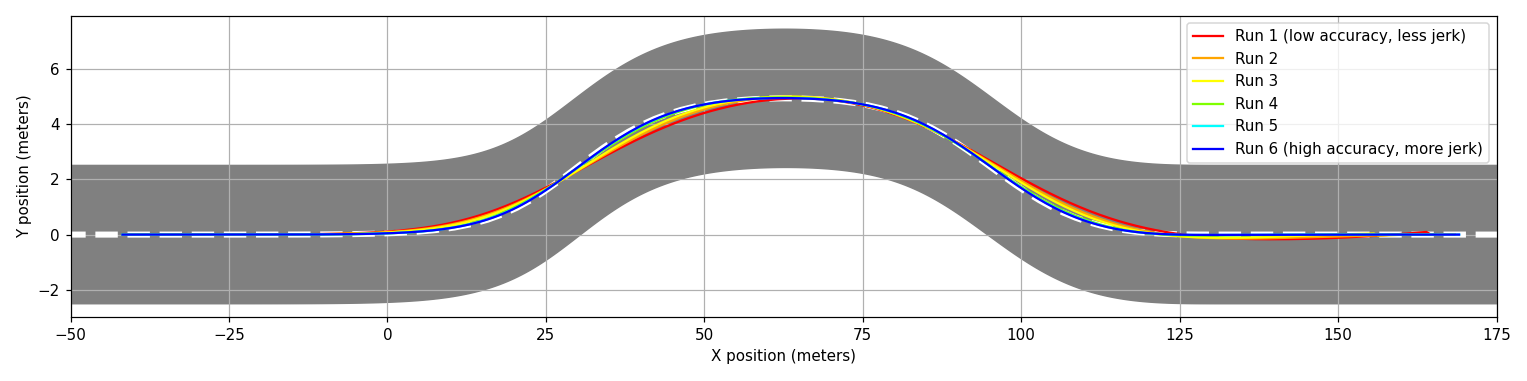
\includegraphics[width=1.0\linewidth]{figures/road_paths.png}
\end{figure}
\vspace{-0.5em}

\begin{table}
	\begin{tabular}{c|cccccc}
Run & 1 & 2 & 3 & 4 & 5 & 6
\\\hline
 $J_{accuracy}$ & 0.01 & 0.05 & 0.1 & 1.0 & 5.0 & 10.0
\\
 $J_{speed}$ & 0.1 & 0.5 & 1.0 & 10.0 & 50.0 & 100.0
\end{tabular}
\end{table}

\end{frame}

\begin{frame}
\frametitle{Performance on ISO Lane Change}

As expected, the magnitude of the steering input increases to keep the vehicle closer to the road center.
\vspace{-0.5em}
\begin{figure}
	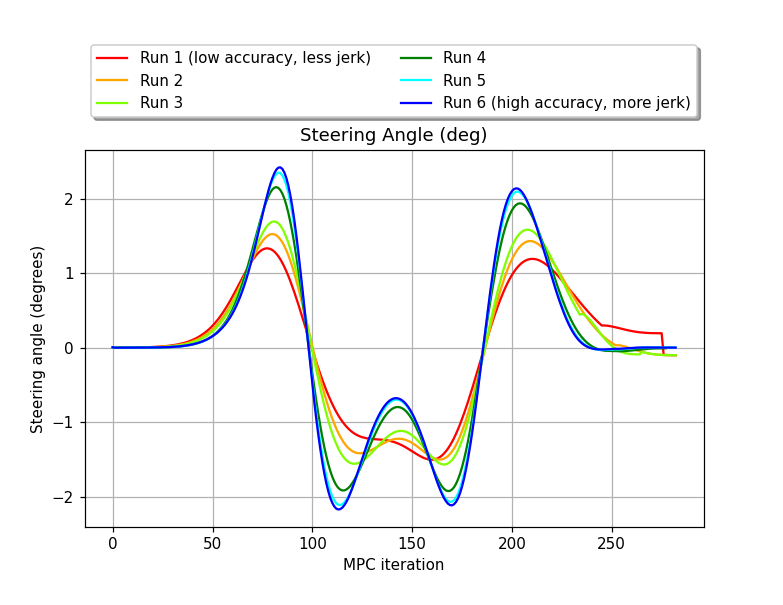
\includegraphics[width=0.8\linewidth]{figures/steering_angle.png}
\end{figure}
\vspace{-0.5em}
\small
\begin{table}
	\begin{tabular}{c|cccccc}
		Run & 1 & 2 & 3 & 4 & 5 & 6
		\\\hline
		$J_{accuracy}$ & 0.01 & 0.05 & 0.1 & 1.0 & 5.0 & 10.0
		\\
		$J_{speed}$ & 0.1 & 0.5 & 1.0 & 10.0 & 50.0 & 100.0
	\end{tabular}
\end{table}
\normalsize
\end{frame}

\begin{frame}
\frametitle{Changing Model Parameters}

The kinematic bicycle model has only 2 parameters describing the distances between the rear/front axles and the vehicle CG.

\vspace{-0.5em}
\begin{figure}
	\centering
	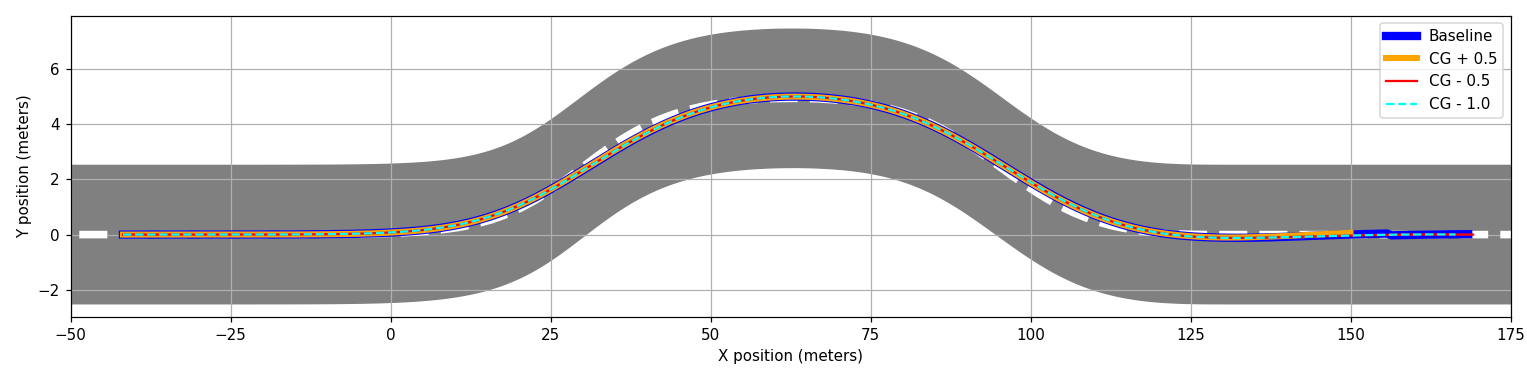
\includegraphics[width=1.0\linewidth]{figures/road_paths_cg.png}
\end{figure}


Changing these parameters does not destabilize the system, though larger control inputs are required to keep the vehicle on the path.

All 3 runs were computed with cost:
$$J = J_{accuracy} + 10 J_{speed} + 100J_{jerk} + 10\frac{180}{\pi} J_{steering}$$
which corresponds to the ``mid-range" performance seen on the previous graphs.
\end{frame}

\begin{frame}
\frametitle{Changing Model Parameters}

When the CG is pushed forward or back, as expected, larger control inputs are generated.

\vspace{-0.5em}
\begin{figure}
	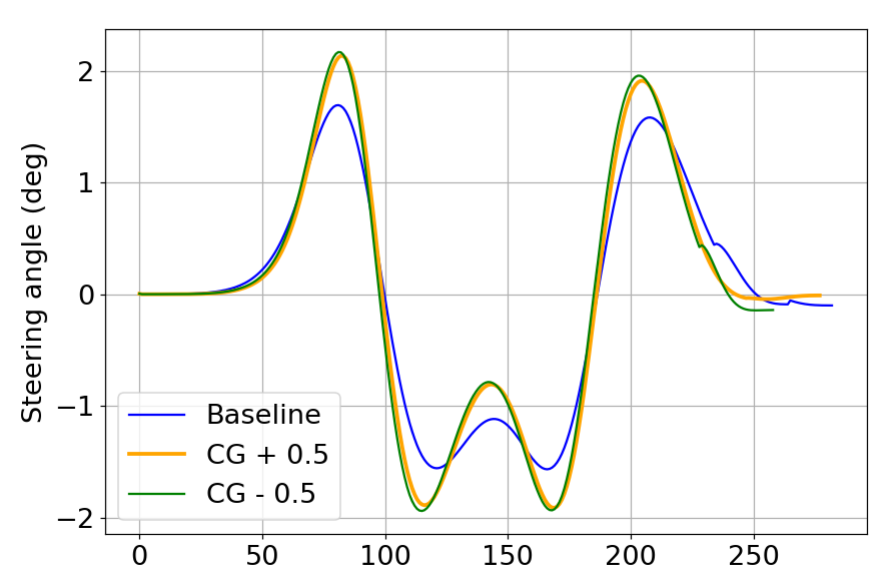
\includegraphics[width=0.75\linewidth]{figures/steering_angle_cg.png}
\end{figure}
\vspace{-0.5em}

This proof of concept shows how the controller could improve software reusability. A high-level autonomous system providing instructions to this optimizing controller does not have to ``know" about the change in CG.
\end{frame}

\begin{frame}
\frametitle{Summary}
\textbf{Current accomplishments:}
\begin{itemize}
	\item Programmed a nonlinear MPC controller for vehicle steering and longitudinal acceleration
	\item Demonstrated ability to easily change vehicle parameters
	\item Configurable driving behavior via weighted multiobjective cost function.
\end{itemize}

\textbf{Potential research directions:}
\begin{itemize}
	\item Faster and more reliable methods of solving nonlinear MPC problems.
\begin{itemize}
	\item Dimensional lifting for linearization?
\end{itemize}
\item Real-time estimation: vehicle parameters can change slowly (tire degradation, temperature change), rapidly (driving into a puddle or patch of ice) and while parked (loading/unloading heavy cargo).
\end{itemize}

\end{frame}

\begin{frame}
\vspace{8.0em}
\begin{center}
\Huge{Questions?}\normalsize
\vspace{1.0em}
\begin{figure}[b!]
	\centering
	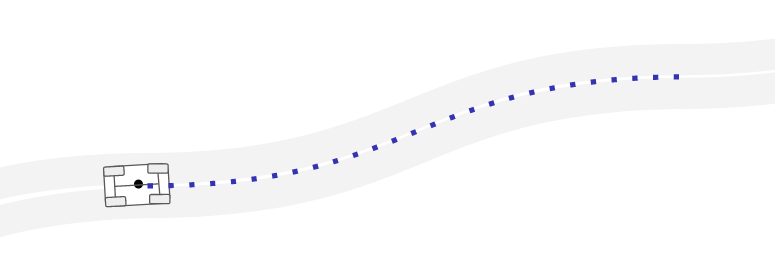
\includegraphics[width=1.0\linewidth]{figures/end_slide.png}
\end{figure}
\end{center}
\end{frame}
	
% Why we can succeed now?
%\begin{frame}
%\frametitle{Reliable Trajectory Optimization}

%Nonlinear optimization algorithms aren't guaranteed to produce an optimal result and can fail unexpectedly: undesirable behavior in a safety-critical application such as autonomous driving.

%Many approaches seek to eliminate nonlinearity.
%\begin{itemize}
%	\item
%Taylor approximation: linearize around a nominal trajectory. If the cost is quadratic, this produces a convex problem that can be quickly and reliably solved.

%However, if the solution strays too far from the nominal trajectory, it is inaccurate. Local approximations also lose information about the system dynamics.

%\item Feedback linearization: 

%\item Koopman linearization: a dimensional lifting method that approximates a nonlinear problem as an infinite-dimensional linear problem.
%\end{itemize}
%\end{frame}

% 4.Are there others dedicated to finding a solution to the problem?

%\begin{frame}
%\frametitle{Recent work in trajectory optimization}

%\end{frame}

% 5.What is the impact if successful?
	
\end{document}